\begin{figure*}
  \centering
  % \begin{noindent}
  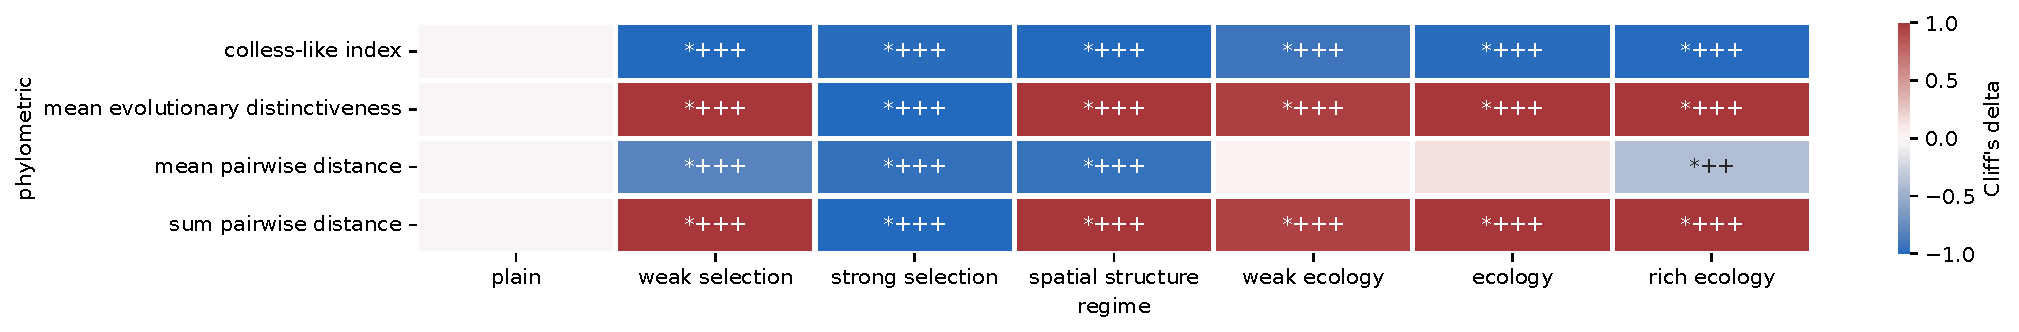
\includegraphics[width=0.5\textwidth]{binder/binder/teeplots/epoch=7+mut_distn=np.random.standard_normal+viz=heatmap+x=regime+y=phylometric+ext=.pdf}
  % 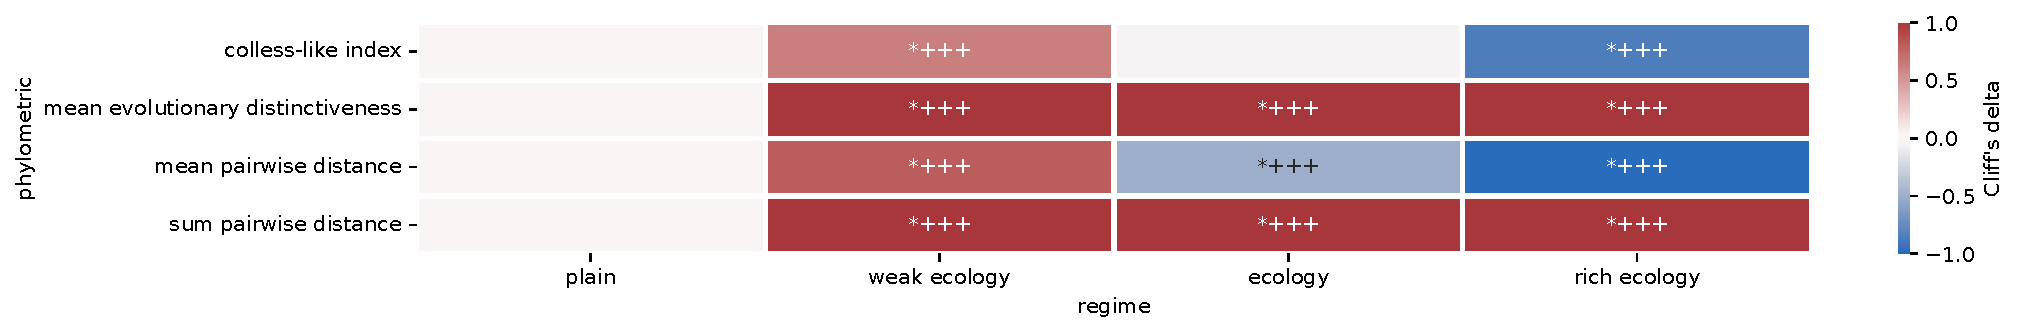
\includegraphics[width=0.5\textwidth]{binder/binder/teeplots/epoch=7+mut_distn=np.random.standard_normal+spatial=true+viz=heatmap+x=regime+y=phylometric+ext=.pdf}
  % \end{noindent}
  \caption{%
  \textbf{Phylometrics in Gen3sis.}
   Evolutionary regimes' effect sizes relative to ``plain'' baseline under the Gen3sis model with perfect phylogenetic tracking, normalized via Cliff's delta.
    Sample sizes $n=30$.
  }
\end{figure*}
